\documentclass[runningheads]{llncs}
\usepackage[T1]{fontenc}
\usepackage[utf8]{inputenc}
\usepackage[polish]{babel}
\usepackage{amsmath,amssymb}
\usepackage{graphicx}
\usepackage{booktabs}
\usepackage{multirow}
\usepackage[hidelinks,pdfauthor={},pdftitle={}]{hyperref}

\begin{document}

\title{Głębokość czy shoty? Liczba warstw QAOA w kwantowym przeszukiwaniu
sąsiedztwa dla permutacyjnego problemu przepływowego}
\titlerunning{Głębokość czy shoty?}
\author{Anonim}
\institute{Anonim}
\maketitle

\begin{abstract}
Kwantowe przeszukiwanie sąsiedztwa wybiera ruch w szeregowaniu, próbkując
obwód QAOA i zachowując próbkę o najniższej energii. Dotychczasowe prace nad
permutacyjnym problemem przepływowym na komputerach bramkowych używały jednej
warstwy QAOA i nie wiadomo, ilu warstw takie sąsiedztwo potrzebuje.
Zmieniamy głębokość $p$ od 1 do 10 w czterech sąsiedztwach (Adjacent,
Fibonacci, Dynasearch i Motzkin) przy kątach stałych skalibrowanych na
trzech rodzajach okien treningowych. Mierzymy jej wpływ na
prawdopodobieństwo wylosowania ruchu optymalnego, na koszt obwodu i na
długość uszeregowania, którą osiąga iteracyjne przeszukiwanie lokalne na
instancjach Taillarda z 20 zadaniami. Bez szumu $p = 1$ jest w dwóch
sąsiedztwach gorsze od losowania jednostajnego. Już przy $p = 2$ najlepsza
z 4096 próbek jest optymalna prawie w każdym oknie sąsiedztw gęstych,
a mediana odchylenia od dolnego ograniczenia spada przy 256 shotach
z około 24\% do 15\%.
W sąsiedztwach liniowych losowanie jednostajne jest tak samo dobre jak każda
głębokość. Na symulowanym 16-kubitowym procesorze o topologii gwiazdy ze
skalibrowanym szumem najlepsza głębokość sąsiedztw gęstych to $p = 2$,
a każda kolejna
warstwa, licząca około 150 bramek dwukubitowych, zbliża trafienia
z powrotem do poziomu losowania jednostajnego. Na samym urządzeniu $p = 1$
zachowuje się jak losowanie jednostajne.
% H2: tu zdanie o p = 2 i 3 na Siriusie
Pochodzenie kątów waży więcej niż głębokość, a średnia energia, którą
minimalizuje kalibracja, słabo przewiduje trafianie optimum.
\keywords{QAOA \and głębokość obwodu \and problem przepływowy \and przeszukiwanie sąsiedztwa \and kąty stałe}
\end{abstract}

\section{Wstęp}

Permutacyjny problem przepływowy (PFSP) polega na wyznaczeniu kolejności
$n$ zadań przechodzących przez $m$ maszyn tak, aby ostatnie zadanie
zakończyło się jak najwcześniej. Standardowym zbiorem testowym pozostają
instancje Taillarda~\cite{taillard1993}. Iteracyjne przeszukiwanie
lokalne~\cite{lourenco2003} radzi sobie z tym problemem dobrze, gdy
sąsiedztwo jest duże. Sąsiedztwa wykładnicze, takie jak sąsiedztwo
Fibonacciego Bożejki i in.~\cite{bozejko2026new} i sąsiedztwo Motzkina
Wojewódzkiego i Bożejki~\cite{wojewodzki2026soco,wojewodzki2025exit},
zawierają znacznie więcej ruchów, niż da się wypisać. Najlepszy ruch trzeba
więc znaleźć, rozwiązując problem optymalizacyjny, programowaniem
dynamicznym albo przez ocenę hybrydową~\cite{wojewodzki2026icaisc}.

Wybór najlepszej kombinacji zamian można zapisać jako
QUBO~\cite{lucas2014ising}, więc wybór ruchu jest naturalnym zadaniem dla
sprzętu kwantowego. Na wyżarzaczach kwantowych te sąsiedztwa oceniano
w iteracyjnym przeszukiwaniu lokalnym i w symulowanym
wyżarzaniu~\cite{wojewodzki2026bpasts}, a okienkowa dekompozycja QUBO
rozszerza to podejście na instancje do 500 zadań~\cite{wojewodzki2026windowed}.
Na procesorach bramkowych to samo QUBO próbkuje się algorytmem
QAOA~\cite{farhi2014qaoa}. Bożejko i in.~\cite{bozejko2024cinti}
zastosowali hybrydowe kwantowe algorytmy aproksymacyjne do problemu
przepływowego, a QAOA o stałych kątach z sąsiedztwami okienkowymi
uruchomiono na procesorach IBM i IQM~\cite{wojewodzki2026gcmm,wojewodzki2026aciids}.
W tym zastosowaniu przeszukiwanie lokalne nie potrzebuje oczekiwanej energii
stanu QAOA. Potrzebuje jednej dobrej próbki, czyli przypisania o najniższej
energii spośród $S$ shotów.

Wszystkie dotychczasowe prace o sąsiedztwach na komputerach bramkowych
używały jednej warstwy QAOA. Literatura o głębokości dotyczy problemu MaxCut
i modelu Sherringtona--Kirkpatricka~\cite{zhou2020,basso2022,wurtz2021fixed}
i mierzy koszt oczekiwany, a nie najlepszą ze skończonej liczby próbek
w pętli przeszukiwania. Dudkiewicz~\cite{dudkiewicz2026depth} zmieniał
głębokość w wielowymiarowym problemie plecakowym, z kątami optymalizowanymi
przez COBYLA i inną miarą jakości. Otwarte pozostaje więc pytanie, czy
sąsiedztwo w szeregowaniu zyskuje na głębszych obwodach i czy szum zostawia
na nie miejsce.

Niniejsza praca bada głębokość $p$ QAOA o stałych kątach w czterech
sąsiedztwach PFSP. Kalibrujemy kąty dla $p = 1, \dots, 10$ na trzech
rodzajach okien treningowych i mierzymy bez szumu, jak często obwód losuje
ruch optymalny w oknach, które buduje przeszukiwanie lokalne. Następnie
sprawdzamy, czy stały budżet lepiej wydać na więcej warstw, czy na więcej
shotów, i wyznaczamy najlepszą głębokość przy skalibrowanym szumie
16-kubitowego procesora o topologii gwiazdy. Na koniec przenosimy wyniki
z okien na długość uszeregowania w iteracyjnym przeszukiwaniu lokalnym na
instancjach Taillarda z 20 zadaniami. Punktami odniesienia są losowanie
jednostajne ($p = 0$) i dokładne klasyczne przeszukiwanie sąsiedztwa.
% H2: tu zdanie o p = 2 i 3 na Siriusie
Przebiegi sprzętowe przy $p = 1$ pochodzą z wcześniejszej kampanii na
procesorze IQM Sirius~\cite{wojewodzki2026aciids}.

\section{Przegląd literatury}

Farhi i in.~\cite{farhi2014qaoa} zaproponowali kwantowy algorytm
aproksymacyjny (QAOA), który przeplata $p$ warstw hamiltonianu kosztu
i hamiltonianu miksującego, a przy rosnącym $p$ zbliża się do ewolucji
adiabatycznej. Zhou i in.~\cite{zhou2020} wykazali, że optymalne kąty zmieniają
się z $p$ w sposób gładki, i zaproponowali regułę INTERP, która buduje
harmonogram dla głębokości $p+1$ przez interpolację harmonogramu dla $p$.
Basso i in.~\cite{basso2022} ocenili QAOA przy głębokościach znacznie większych
niż $p = 1$ na grafach regularnych o dużej talii, a Wurtz i
Łykow~\cite{wurtz2021fixed} podali kąty stałe dla grafów regularnych w
problemie MaxCut, które nie wymagają optymalizacji dla każdej instancji.
Wszystkie te wyniki dotyczą MaxCut lub modelu Sherringtona--Kirkpatricka
i odczytują oczekiwany koszt stanu QAOA, a nie najlepszą ze skończonej liczby
próbek.

Szum ogranicza głębokość użytecznego obwodu. Stilck Fran\c{c}a
i Garc\'{i}a-Patr\'{o}n~\cite{franca2021} pokazali, że na zaszumionych
urządzeniach wynik algorytmów wariacyjnych przy dostatecznie głębokim obwodzie
zbliża się do stanu, któremu dorównują wydajne metody klasyczne. Harrigan
i in.~\cite{harrigan2021} uruchomili QAOA na procesorze nadprzewodzącym
i stwierdzili, że dla problemów, których graf nie pasuje do układu, routing
dokłada bramki, a jakość spada wraz z rozmiarem problemu. Gnatowski
i in.~\cite{gnatowski2026routing} podali dokładny algorytm routingu dla
architektur gwiaździstych, czyli topologii procesora użytego w tej pracy.

\section{Kwantowe przeszukiwanie sąsiedztwa}

W permutacyjnym problemie przepływowym (PFSP) $n$ zadań przechodzi przez $m$
maszyn w tej samej kolejności, a permutacja $\pi$ ustala kolejność zadań na
każdej maszynie. Celem jest minimalizacja długości uszeregowania
$C_{\max}(\pi)$, czyli chwili zakończenia ostatniego zadania na ostatniej
maszynie. Iteracyjne przeszukiwanie lokalne (ILS)~\cite{lourenco2003}
przechodzi od $\pi$ do najlepszej permutacji w sąsiedztwie $N(\pi)$
i zaburza $\pi$, gdy przestaje ona się poprawiać.

Ruch w badanych sąsiedztwach to zbiór rozłącznych zamian. Każda kandydująca
zamiana $k$ ma wcześniej policzoną zmianę długości uszeregowania $\Delta_k$,
a zmienna binarna $x_k$ ją wybiera. QUBO wyboru zamian~\cite{lucas2014ising}
\begin{equation}
  E(x) = \sum_k \Delta_k x_k + P \sum_{(k,l) \in \mathcal{C}} x_k x_l ,
  \qquad P = 1 + \sum_k |\Delta_k| ,
\end{equation}
sumuje zmiany wybranych zamian i nakłada karę na każdą parę ze zbioru
konfliktów $\mathcal{C}$, więc każde przypisanie łamiące ograniczenie kosztuje
więcej niż brak ruchu. Tabela~\ref{tab:neigh} zestawia cztery sąsiedztwa.
Adjacent wybiera dokładnie jedną zamianę sąsiadów i ma QUBO typu one-hot
z $Q_{ii} = \Delta_i - P$, $Q_{ij} = 2P$ oraz $P = 2\max_i|\Delta_i| + 1$.
Sąsiedztwo Fibonacciego~\cite{bozejko2026new} dopuszcza dowolny zbiór
rozłącznych zamian sąsiednich, co daje QUBO trójdiagonalne. Dynasearch
i sąsiedztwo Motzkina~\cite{wojewodzki2026soco} zamieniają końce przedziałów;
Dynasearch zabrania nakładania się przedziałów, Motzkin dopuszcza też ich
zagnieżdżanie, a oba dają QUBO z konfliktami parami.

\begin{table}[t]
\caption{Cztery sąsiedztwa ($F_{n+1}$, $M_n$: liczby Fibonacciego
i Motzkina; ostatnia kolumna: zmienne na okno w ILS, $n = 20$).}
\label{tab:neigh}
\centering
\begin{tabular}{lllll}
\toprule
Sąsiedztwo & Ruch & Ruchów & QUBO & Zmiennych na okno \\
\midrule
Adjacent   & jedna zamiana sąsiednia          & $n - 1$   & one-hot       & 1--16 (mediana 10) \\
Fibonacci  & rozłączne zamiany sąsiednie      & $F_{n+1}$ & trójdiagonalne & 1--16 (mediana 10) \\
Dynasearch & rozłączne zamiany końców przedz. & $2^{n-1}$ & parami        & 4--15 (mediana 14) \\
Motzkin    & nieprzecinające się przedziały   & $M_n$     & parami        & 4--15 (mediana 14) \\
\bottomrule
\end{tabular}
\end{table}

Cała permutacja $n = 20$ zadań daje więcej zmiennych, niż mieści procesor
16-kubitowy, dlatego ILS dzieli permutację na nakładające się okna po $w$
pozycji z nakładaniem $0{,}5$ i rozwiązuje jedno QUBO na
okno~\cite{wojewodzki2026windowed,wojewodzki2026aciids}. Okno ma $w = 17$
pozycji dla sąsiedztw liniowych i $w = 6$ dla gęstych. W sąsiedztwach
liniowych ILS zostawia tylko kandydatów, których akcelerator bloków uznaje za
zdolnych poprawić $C_{\max}$, więc ich okna mają na instancjach Taillarda
z $n = 20$ od 1 do 16 zmiennych (mediana 10), a okna gęste od 4 do 15
(mediana 14).

\section{QAOA o głębokości $p$}

Podstawienie $x_k = (1 - Z_k)/2$ zamienia $E(x)$ w hamiltonian Isinga
$H_C = \sum_k h_k Z_k + \sum_{k<l} J_{kl} Z_k Z_l$, który skalujemy tak,
aby jego największy współczynnik miał moduł jeden. Stan QAOA o głębokości
$p$ ma postać
\begin{equation}
  |\gamma,\beta\rangle = \prod_{\ell=1}^{p}
  e^{-i\beta_\ell H_M} e^{-i\gamma_\ell H_C} \, |{+}\rangle^{\otimes K},
  \qquad H_M = \sum_k X_k ,
\end{equation}
a każda warstwa kosztuje jedną bramkę $R_{ZZ}$ na sprzężenie oraz po jednej
bramce $R_Z$ i $R_X$ na kubit.

Kąty ustalamy z góry, więc każdy ruch kosztuje jedno wykonanie obwodu. Dla
każdego sąsiedztwa kalibrujemy jeden harmonogram
$(\gamma_1, \dots, \gamma_p, \beta_1, \dots, \beta_p)$ na głębokość,
minimalizując średnią z
$\langle H_C \rangle / (\sum_k |h_k| + \sum_{k<l} |J_{kl}|)$ na zbiorze
treningowym okien z trzech instancji Taillarda~\cite{taillard1993}. Przy
$p = 1$ minimum znajduje siatka $25 \times 13$ po $\gamma \in [0, \pi]$
i $\beta \in [0, \pi/2]$. Dla $p \ge 2$ metoda Neldera--Meada startuje
z czterech harmonogramów: harmonogramu dla $p-1$ z pustą ostatnią warstwą,
który nie pozwala funkcji celu wzrosnąć, jego przepróbkowania
INTERP~\cite{zhou2020} oraz dwóch jego zaburzonych kopii, z budżetem $400p$
iteracji. Funkcja celu nie rośnie więc z $p$ na zbiorze treningowym, co nie
mówi nic o oknach spoza niego. Budujemy trzy tabele, które różnią się tylko
oknami treningowymi: \emph{małe} okna o $w = 6$ pozycjach ($p \le 10$),
\emph{duże} okna o rozmiarach z ILS bez akceleratora bloków ($p \le 5$) oraz
okna przechwycone z samego ILS ($p \le 5$). Dla sąsiedztw gęstych dwie
ostatnie się pokrywają.

ILS próbkuje obwód $S$ razy i wybiera próbkę o najniższej energii
pierwotnego QUBO. Wybór najczęstszego ciągu bitów zwracałby często pusty
ruch. Jeśli $P_{\mathrm{opt}}$ to prawdopodobieństwo przypisania optymalnego,
najlepsza z $S$ próbek jest optymalna z prawdopodobieństwem
$1 - (1 - P_{\mathrm{opt}})^S$, więc więcej shotów może nadrobić słabszy
rozkład.

W procesorze o topologii gwiazdy każdy kubit jest sprzężony tylko
z centralnym rezonatorem, a oddziaływanie dwukubitowe wymaga najpierw
przeniesienia stanu jednego kubitu do rezonatora. Jedna bramka $R_{ZZ}$
kompiluje się wtedy do dwóch bramek CZ i około dwóch bramek
MOVE~\cite{gnatowski2026routing}, więc gęste okno z 15 zmiennymi potrzebuje
150 bramek CZ na warstwę, pięć razy więcej niż okno liniowe z 15 sprzężeniami,
a koszt rośnie liniowo z $p$.

\section{Plan eksperymentów}

Wszystkie eksperymenty korzystają z instancji Taillarda z $n = 20$
zadaniami i $m \in \{5, 10, 20\}$ maszynami, po dziesięć instancji w każdej
klasie~\cite{taillard1993}, a ILS startuje z permutacji tożsamościowej, jak
we wcześniejszej kampanii~\cite{wojewodzki2026aciids}. QAOA oceniamy na
trzech poziomach. Na poziomie bez szumu obwód jest próbkowany z dokładnego
wektora stanu. Na poziomie z szumem symulowany 16-kubitowy procesor
o topologii gwiazdy odtwarza wierności bramek i błędy odczytu, które IQM
podało dla procesora Sirius 23~października~2026; w trybie domyślnym każda
bramka jednokubitowa i CZ ma dokładnie zmierzoną wierność, a drugi tryb
dodaje relaksację $T_1$/$T_2$, która sama przekracza zmierzony błąd
większości bramek. Żaden z trybów nie nakłada szumu na bramki MOVE. Na
poziomie sprzętowym obwody wykonuje sam Sirius.

Badanie okien odczytuje rozkład QAOA dla pojedynczych okien. Przechwytujemy
okna pierwszego ruchu ILS z permutacji tożsamościowej i z dwóch losowych
permutacji każdej instancji, łącznie 1440 okien, z których 1195 zawiera ruch
poprawiający, i wyznaczamy ich optimum przez pełne przeszukanie. Poziom bez
szumu daje $P_{\mathrm{opt}}$ dokładnie dla $p = 0, \dots, 10$; poziom
z szumem próbkuje okna instancji 0--3 przy 4096 shotach dla
$p = 0, \dots, 6$.

Badanie ILS mierzy długość uszeregowania. Bez szumu ILS działa przez 10~s
w czterech wariantach: QAOA z tabelą z małych okien dla $p = 1, \dots, 10$,
QAOA z najlepszą tabelą z badania okien dla sąsiedztw liniowych ($p \le 5$),
$p = 0$, czyli losowanie jednostajne z tym samym odczytem najniższej energii,
oraz klasyczne przeszukiwanie sąsiedztwa, które ocenia każdy ruch dokładnie.
Warianty QAOA używają $S = 256$ i $S = 4096$ shotów. Sąsiedztwa liniowe
uruchamiamy raz na instancję, a gęste pięć razy. Symulator z szumem
potrzebuje minut na obwód, więc jego czas nie mówi nic o urządzeniu; każdy
przebieg z szumem wykonuje więc dokładnie tyle ruchów, ile Sirius wykonał
w 10~s na tej samej instancji przy $p = 1$~\cite{wojewodzki2026aciids}. Na
sprzęcie ILS powtarza tamtą kampanię dla $p = 2$ i $p = 3$.
% H2: zdanie prawdziwe dopiero po biegach na Siriusie (p = 2, 3)

Podajemy procentowe odchylenie względne
$\mathrm{PRD} = 100\,(C_{\max} - LB)/LB$ od dolnego ograniczenia Taillarda
$LB$, uśredniamy je po przebiegach instancji, bierzemy medianę po
instancjach i porównujemy dwa ustawienia testem znaków par po instancjach.
Każdy przebieg ma ziarno wyznaczone z jego konfiguracji, które ustala
zaburzenia ILS, a bez szumu także losowanie shotów.

\section{Wyniki}

Bez szumu jedna warstwa nie wystarcza (rys.~\ref{fig:e1}). Przy $p = 1$
tylko Adjacent losuje ruch optymalny wyraźnie częściej niż losowanie
jednostajne. Motzkin ledwie je wyprzedza, a Fibonacci i Dynasearch wypadają
poniżej niego. W sąsiedztwach
gęstych płytki obwód faworyzuje przypisania łamiące warunek rozłączności. Od
$p = 2$ sąsiedztwa gęste losują optimum mniej więcej sto razy częściej niż
losowanie jednostajne, a przy 4096 shotach najlepsza próbka jest wtedy
prawie zawsze optymalna (rys.~\ref{fig:hits}). Kolejne warstwy niewiele więc
dodają, a ich miejsce mogą zająć shoty. Zysk nie rośnie jednak monotonicznie
z $p$, a najlepsza tabela kątów zależy od sąsiedztwa: kąty o niższej średniej
energii na oknach treningowych nie muszą częściej znajdować optimum.

Każda warstwa dokłada tyle samo bramek dwukubitowych (tabela~\ref{tab:e3}),
w oknie gęstym mniej więcej dziesięć razy więcej niż w oknie Fibonacciego.
Z szumem ten koszt wyznacza najlepszą głębokość (rys.~\ref{fig:e4}).
W sąsiedztwach gęstych najlepsza próbka jest optymalna najczęściej przy
$p = 2$, a przy $p = 6$ obwód nie jest lepszy od losowania jednostajnego.
Sąsiedztwa liniowe prawie nie odczuwają szumu, bo ich obwody są płytkie,
a losowanie jednostajne i tak znajduje większość optimów.

Ten sam obraz widać w długości uszeregowania w ILS (tabela~\ref{tab:e5}).
Przy 256 shotach $p = 2$ obniża w sąsiedztwach gęstych medianę odchylenia
od dolnego ograniczenia z około 24\% przy losowaniu jednostajnym do 15\%,
a najlepsza głębokość wygrywa z losowaniem jednostajnym na wszystkich 30
instancjach. Przy 4096 shotach wygrywa nadal prawie na wszystkich. Głębsze obwody
przegrywają tylko dlatego, że każdy ruch trwa dłużej i w 10~s mieści się
mniej ruchów (rys.~\ref{fig:moves}). W sąsiedztwach liniowych głębokość nic
nie daje, a klasyczne przeszukiwanie, które ocenia każdy ruch dokładnie,
pozostaje lepsze od wszystkich wariantów QAOA.

Po jednym do trzech ruchach, które Sirius wykonuje w 10~s, większość różnic
w tabeli~\ref{tab:hw} jest niewielka. Na symulatorze z szumem Dynasearch przy
$p = 2$ znów wygrywa z $p = 1$, na 11 z 12 instancji. W Dynasearch przy $p = 1$ urządzenie
radzi sobie lepiej niż symulator i mniej więcej tak samo jak losowanie
jednostajne, co sugeruje, że prawdziwy szum jest silniejszy niż skalibrowany
model. \emph{[H2: czy zysk z $p = 2$ utrzymuje się na Siriusie.]}

\begin{figure}[t]
\centering
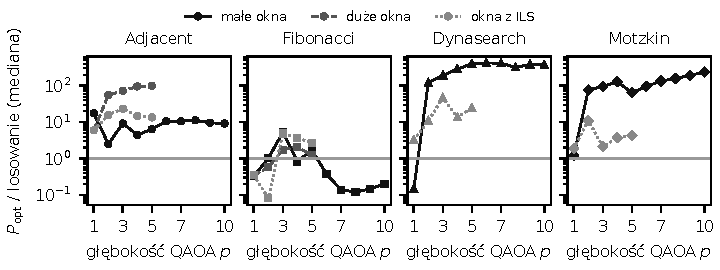
\includegraphics[width=\textwidth]{figures/fig1_e1_pl.pdf}
\caption{$P_{\mathrm{opt}}$ względem losowania jednostajnego w funkcji $p$
dla trzech tabel kątów (mediana po oknach z ruchem poprawiającym; bez
szumu).}
\label{fig:e1}
\end{figure}

\begin{figure}[t]
\centering
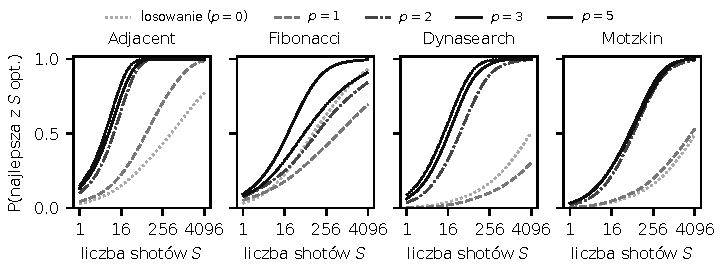
\includegraphics[width=\textwidth]{figures/fig2_hits_pl.pdf}
\caption{Prawdopodobieństwo, że najlepsza z $S$ próbek jest optymalna,
w funkcji $S$ (bez szumu; Adjacent: tabela z dużych okien, pozostałe:
z małych okien).}
\label{fig:hits}
\end{figure}

\begin{table}[t]
\caption{Bramki CZ na okno po kompilacji (mediana po 192 oknach z ILS).}
\label{tab:e3}
\centering
\begin{tabular}{lrrrrrrrr}
\toprule
 & \multicolumn{2}{c}{$p = 1$} & \multicolumn{2}{c}{$p = 3$} & \multicolumn{2}{c}{$p = 6$} & \multicolumn{2}{c}{$p = 10$} \\
\cmidrule(lr){2-3}\cmidrule(lr){4-5}\cmidrule(lr){6-7}\cmidrule(lr){8-9}
Sąsiedztwo & gwiazda & krata & gwiazda & krata & gwiazda & krata & gwiazda & krata \\
\midrule
\csname @@input\endcsname tables/tab1_e3.tex 
\bottomrule
\end{tabular}
\end{table}

\begin{figure}[t]
\centering
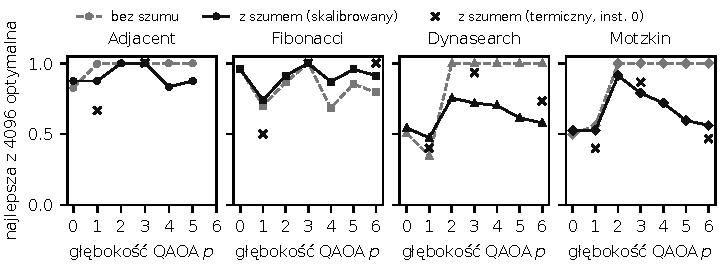
\includegraphics[width=\textwidth]{figures/fig3_noise_pl.pdf}
\caption{Odsetek okien, w których najlepsza z 4096 próbek jest optymalna,
w funkcji $p$ (instancje 0--3; szum termiczny: instancja 0; tabele kątów
jak na rys.~\ref{fig:hits}).}
\label{fig:e4}
\end{figure}

\begin{table}[t]
\caption{ILS bez szumu, 10~s: mediana PRD [\%] po 30 instancjach (tabela
z małych okien; klasyczne: dokładne przeszukiwanie sąsiedztwa).}
\label{tab:e5}
\centering
\begin{tabular}{llrrrrrrr}
\toprule
Sąsiedztwo & $S$ & $p=0$ & $p=1$ & $p=2$ & $p=3$ & $p=6$ & $p=10$ & klasyczne \\
\midrule
\csname @@input\endcsname tables/tab2_prd_pl.tex 
\bottomrule
\end{tabular}
\end{table}

\begin{table}[t]
\caption{Mediana PRD [\%] na instancjach 0--3 po tylu ruchach, ile Sirius
wykonał w 10~s ($S = 4096$; \textbf{?}: w toku; --: nie uruchamiano).}
\label{tab:hw}
\centering
\begin{tabular}{llrrrrr}
\toprule
Sąsiedztwo & poziom & $p=0$ & $p=1$ & $p=2$ & $p=3$ & $p=6$ \\
\midrule
\csname @@input\endcsname tables/tab3_hw_pl.tex 
\bottomrule
\end{tabular}
\end{table}

\begin{figure}[t]
\centering
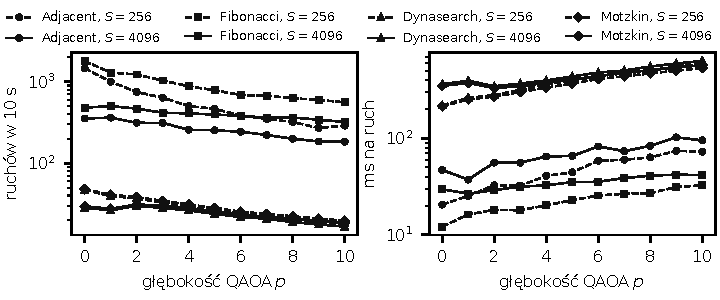
\includegraphics[width=\textwidth]{figures/fig4_moves_pl.pdf}
\caption{Liczba ruchów w 10~s i czas ruchu w funkcji $p$ (bez szumu;
$p = 0$: losowanie jednostajne).}
\label{fig:moves}
\end{figure}

\section{Dyskusja i wnioski}

Jedna warstwa QAOA jest za słaba dla przeszukiwania sąsiedztwa w problemie
przepływowym. Bez szumu dwie warstwy znajdują ruch optymalny prawie w każdym
oknie gęstym, a z szumem $p = 2$ jest też najlepszą głębokością, bo każda
kolejna warstwa kosztuje około 150 bramek dwukubitowych. W sąsiedztwach
liniowych okna są tak małe, że losowanie jednostajne radzi sobie tak samo
dobrze jak QAOA. Dla sąsiedztw gęstych zalecamy więc dwie warstwy
i przeznaczenie reszty budżetu na shoty.
% H2: zalecenie "dwie warstwy" opiera się na symulatorze; złagodzić, jeśli Sirius przy p = 2 nie pokaże zysku
Kąty ważą więcej niż głębokość, a kalibracja na średnią energię nie nagradza
tego, czego potrzebuje przeszukiwanie lokalne.

Nie twierdzimy, że obliczenia kwantowe mają tu przewagę nad klasycznymi:
dokładne przeszukiwanie klasyczne pozostaje wyraźnie lepsze, a na urządzeniu
ILS wykonuje w 10~s tylko od jednego do trzech ruchów. Badanie obejmuje tylko 20
zadań i kąty stałe, a energia okna jest dokładna tylko wtedy, gdy zamiany na
siebie nie wpływają. Symulowane urządzenie nie ma szumu na bezczynnych
kubitach ani na bramkach MOVE, co może tłumaczyć, dlaczego Sirius wyglądał na bardziej
zaszumionego niż symulator. W dalszych pracach kąty będą kalibrowane na
prawdopodobieństwo, że najlepsza próbka jest optymalna, a głębokość będzie
dobierana dla każdego okna.

\subsubsection{Podziękowania.} Autorzy korzystali z dużego modelu językowego
przy redagowaniu i poprawianiu części tekstu, pisaniu skryptów eksperymentów
i składzie w LaTeX-u; badania, ich wyniki i ich interpretacja są w całości
dziełem autorów.

\bibliographystyle{splncs04}
\bibliography{references}

\end{document}
